\kapitola{Vlastní práce}
Vlastní práce se skládá ze dvou částí klientská část, která slouží k vizualizaci algoritmu a zobrazení výsledků ze serverové části. Serverová část pro maximální zrychlení simulace. 
\sekce{Simulace}
\podsekce{Fitness funkce}
Fitness funkce je důležitou součástí simulace, která zásadně ovlivňuje chování výsledných agentů a je tedy nutné jí volit vhodně. 
\sekce{Serverová část}
Serverová část vyhodnocuje jednotlivé jedince distribuovaně s pomocí fronty úkolů. Frontu poskytuje knihovna \textbf{bull}, která používá \textbf{redis} pro správu údajů o jednotlivých úkolech.

Cílem byl návrh robustního systému, který v ideálním případě rozloží výpočetní zátěž mezi jednotlivé uzly rovnoměrně. Dalším požadavkem byla možnost odpojení 

\podsekce{Výpočetní cluster}
Ukázalo, že vyhodnocování simulace zabírá neúměrné množství času a to i na nejvýkonnějším dostupném počítači. 
Například vyhodnocení jedné generace populace o 1024 jedincích zabralo ~290 s na nejsilnějším dostupném pc. Z tohoto důvodu bylo rozhodnuto o distribuce výpočetní zátěže mezi více počítačů. Byl vytvořen výpočetní cluster se specifikací popsanou v tabulce \ref{table:hw_table}.
\begin{table}[h!]
	\centering
	\begin{tabular}{|l|c|c|c|}
		\hline 
		Procesor & RAM & Počet & Architektura\\ 
		\hline 
		S5P6818 Octa core & 1 GB & 2 & arm64 \\ 
		\hline 
		Broadcom BCM2837B0 quad-core & 1 GB & 1 & arm32 \\ 
		\hline 
		Phenom X4 965 & 8 GB & 1 & x64 \\ 
		\hline
		Intel Core i5-2300 & 4 GB & 1 & x64 \\ 
		\hline
		AMD A4-4300M & 4 GB & 1 & x64 \\ 
		\hline 
		Intel atom x5-Z8350 & 2 GB & 1 & x64 \\ 
		\hline
	\end{tabular} 
	\caption{Použitý hardware}
	\label{table:hw_table}
\end{table}

\podsekce{Docker swarm}
Pro snadnou distribuci a správu byly všechny počítače zorganizovány do docker swarmu. Docker swarm obsahoval jednoho managera (Broadcom BCM2837B0 quad-core), který zároveň spouštěl klientskou aplikaci a další služby:

\begin{enumerate}
	\item \textbf{Portainer} pro správu clusteru
	\item \textbf{Arena} webové ui pro správu \textbf{bull}
	\item \textbf{redis} používaný knihovnou \textbf{bull}
\end{enumerate}


\podsekce{Průběh vyhodnocování}
Serverová část pracuje dle diagramu \ref{fig:distributed}, kde je vidět, že klient zadává do fronty úkoly (genom a nastavení simulace) a jednotliví zpracovatelé (počítače v clusteru), kteří si je z ní vyberou, jednotlivé genomy vyhodnotí a hodnotu fitness funkce pošlou zpět na klienta, který jakmile dostane všechny hodnoty zpět provede genetický algoritmu (mutace, křížení, ...) a novou generaci pošle znovu na vyhodnocení.
\begin{figure}[h!]
	\centering
	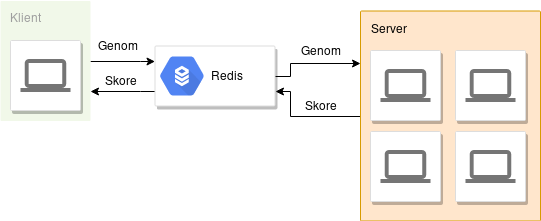
\includegraphics[scale=0.5]{distributed}
	\caption[Schéma distribuovaných výpočtů]{Schéma distribuovaných výpočtů}
	\label{fig:distributed}
\end{figure}
Tento přístup má několik výhod a to:
\begin{enumerate}
	\item Robustnost - Pokud jeden nebo více zpracovatelů selže (je například odpojen ze sítě) je možné pokračovat ve vyhodnocování (neúspěšný úkol se automaticky vrátí zpátky do fronty)
	\item Dobré rozložení zátěže - Jelikož si zpracovatel vytahuje úkoly z fronty je vždy optimálně zatížen a není třeba řešit rozložení mezi různě výkonnými a zatíženými počítači.
	\item Možnost vyhodnocení více úkolů zároveň - Jelikož se vyhodnocují jednotlivé genomy lze spustit i více simulací zároveň bez většího dopadu na výkon výpočtů.
\end{enumerate}

Lze i namítnout, že se zde projevuje určitá režie při síťové komunikaci se serverem, což může být zdrojem určitého zpomalení. Nicméně se toto zpomalení neprojevilo v průběhu testování clusteru. 
\sekce{Klientská část}
\sekce{Simulace}
\podsekce{Agent}
Definice samotného agenta zásadně ovlivňuje výsledek simulace, protože stanovuje vstupy a výstupy do a z neuronové sítě. 

Samotný agent je auto, které je vybaveno 6 vzdálenostními senzory. Měření těchto senzorů je normalizováno (maximální vzdálenost měřícího paprsku je 800 m) a předáno jako vstup do neuronové sítě.

Agent se poté každý snímek s pomocí neuronové sítě rozhoduje, jakou akci podnikne. Má následující možnosti:

\begin{figure}[h!]
	\centering
	\begin{neuralnetwork}[height=7]
		\newcommand{\nodetextx}[2]{\ifthenelse{\equal{#2}{0}}{$b_0$}{$s_{#2}$}}
		\newcommand{\nodetextz}[2]{$z_#2$}
		\newcommand{\nodetexth}[2]{\ifthenelse{\equal{#2}{0}}{$b_1$}{$h_{#2}$}}
		\inputlayer[count=6, title={Data ze senzorů}, text=\nodetextx]
		\hiddenlayer[count=6, title={Skrytá vrstva}]
		\linklayers
		\outputlayer[count=6, title={Výstup}, text=\nodetextz] 
		\linklayers
	\end{neuralnetwork}
	\caption{Neuronová síť agenta}
	\label{fig:control_network}
\end{figure}
 
\sekce{Experimenty}
Po návrhu simulačního prostředí byl agent vyzkoušen v několika situacích se stupňující se obtížností. Každá simulace probíhala s 1000 jedinci po 2000 generací.   
\podsekce{Nekonečná silnice ve tvaru I}
Agent byl umístěn do nekonečné rovné silnice ve tvaru I. Cílem bylo pozorovat, zda se agent bude schopný naučit řídit rovně. 
\begin{figure}
	\centering
	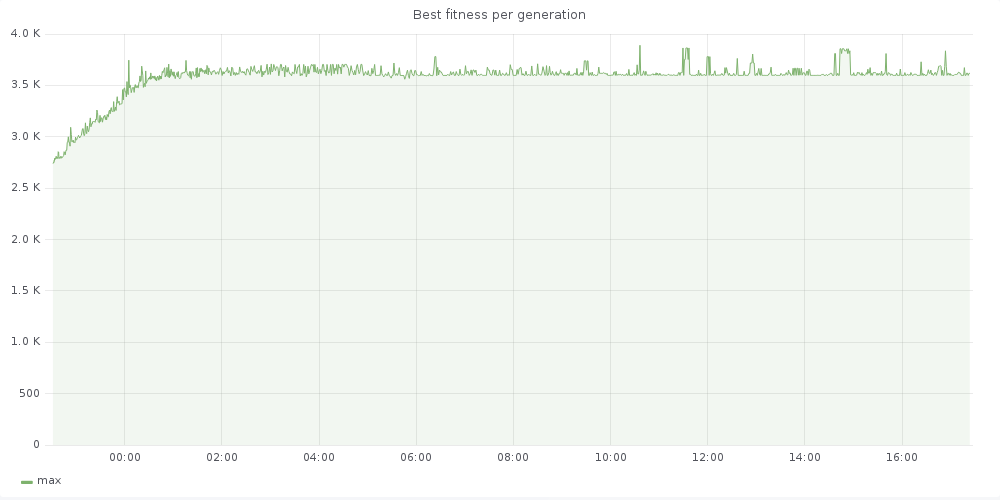
\includegraphics[scale=0.4]{I_fitness}
	\caption{Skore experimentu}
	\label{fig:i-experiment}
\end{figure}

\kapitola{Možná vylepšení}
\kapitola{Závěr} 

https://snapshot.raintank.io/dashboard/snapshot/FmoHRo3sfdk8eAQlkRc4rfKK3YF043oE?orgId=2
https://snapshot.raintank.io/dashboard/snapshot/uDjEpO6qYTv8Sbo0SeJIXJGS4uU1N2hY?orgId=2
https://snapshot.raintank.io/dashboard/snapshot/Lfnfr79JuQEItfU2sOnxWoRHN0m0ckzM?orgId=2